\documentclass{beamer}
\usepackage{subfigure}

% There are many different themes available for Beamer. A comprehensive
% list with examples is given here:
% http://deic.uab.es/~iblanes/beamer_gallery/index_by_theme.html
% You can uncomment the themes below if you would like to use a different
% one:
%\usetheme{AnnArbor}
%\usetheme{Antibes}
%\usetheme{Bergen}
%\usetheme{Berkeley}
%\usetheme{Berlin}
%\usetheme{Boadilla}
%\usetheme{boxes}
%\usetheme{CambridgeUS}
%\usetheme{Copenhagen}
%\usetheme{Darmstadt}
%\usetheme{Frankfurt}
%\usetheme{Goettingen}
%\usetheme{Hannover}
%\usetheme{Ilmenau}
%\usetheme{JuanLesPins}
%\usetheme{Luebeck}
%\usetheme{Madrid}
%\usetheme{Malmoe}
%\usetheme{Marburg}
%\usetheme{Montpellier}
%\usetheme{PaloAlto}
%\usetheme{Pittsburgh}
%\usetheme{Rochester}
%\usetheme{Singapore}
%\usetheme{Szeged}
%\usetheme{Warsaw}

\title{Spatial Reading Group}

% A subtitle is optional and this may be deleted
\subtitle{Optional Subtitle}

%\date{Conference Name, 2013}
% - Either use conference name or its abbreviation.
% - Not really informative to the audience, more for people (including
%   yourself) who are reading the slides online

\subject{blah}
% This is only inserted into the PDF information catalog. Can be left
% out. 

% If you have a file called "university-logo-filename.xxx", where xxx
% is a graphic format that can be processed by latex or pdflatex,
% resp., then you can add a logo as follows:

% \pgfdeclareimage[height=0.5cm]{university-logo}{university-logo-filename}
% \logo{\pgfuseimage{university-logo}}

% Delete this, if you do not want the table of contents to pop up at
% the beginning of each subsection:
\AtBeginSubsection[]
{
  \begin{frame}<beamer>{Outline}
    \tableofcontents[currentsection,currentsubsection]
  \end{frame}
}

% Let's get started
\begin{document}

\begin{frame}
  \titlepage
\end{frame}

\begin{frame}{Outline}
  \tableofcontents
  % You might wish to add the option [pausesections]
\end{frame}

% Section and subsections will appear in the presentation overview
% and table of contents.
\section{First Main Section}

\subsection{First Subsection}

\begin{frame}{First Slide Title}{Optional Subtitle}
  \begin{itemize}
  \item {
    My first point.
  }
  \item {
    My second point.
  }
  \end{itemize}
\end{frame}

\subsection{Second Subsection}

% You can reveal the parts of a slide one at a time
% with the \pause command:
\begin{frame}{Second Slide Title}
  \begin{itemize}
  \item {
    First item.
    \pause % The slide will pause after showing the first item
  }
  \item {   
    Second item.
  }
  % You can also specify when the content should appear
  % by using <n->:
  \item<3-> {
    Third item.
  }
  \item<4-> {
    Fourth item.
  }
  % or you can use the \uncover command to reveal general
  % content (not just \items):
  \item<5-> {
    Fifth item. \uncover<6->{Extra text in the fifth item.}
  }
  \end{itemize}
\end{frame}


\begin{frame}{Kriging}
	\begin{itemize}
		
		\item Suppose our objective is to predict the value of the signal at an arbitrary location $S(x)$.
		
		\item Note that $(S(x), Y)$ is multivariate Gaussian with mean vector $\mu \mathbf{1}$ and covariance matrix
		$$
		\begin{pmatrix}
		\sigma^2 & \sigma^2 r^T\\
		\sigma^2 r & \sigma^2 V
		\end{pmatrix},
		$$
		where $r$ is a vector with elements $r_i = \rho(\|x-x_i\|)$ and $V = \sigma^2 R + \tau^2 I$.
		
		
	\end{itemize}
\end{frame}

\begin{frame}{Kriging}
	\begin{itemize}
		
		\item Conditional mean and variance:
		$$E(S(x) | Y) = \mu + r^T V^{-1}(Y - \mu \mathbf{1}),$$
		$$Var(S(x) | Y) = \sigma^2 (1 - r^T V^{-1} r).$$
		
		\item Two types:
		\begin{itemize} 
			\item Ordinary kriging: replace $\mu$ by its weighted least squares estimator
			$$\hat{\mu} = (\mathbf{1}^T V^{-1} \mathbf{1})^{-1} \mathbf{1}^T V^{-1} Y.$$
			
			\item Simple kriging: replace $\mu$ by $\hat{\mu} = \bar{y}$.
		\end{itemize}
		
		
		
		\item Both kriging predictors can be expressed as a linear combination: $\hat{S}(x) = \sum_{i=1}^{n}a_i(x) Y_i$, but $\sum_{i=1}^{n}a_i(x)=1$ only for ordinary kriging.
	\end{itemize}
\end{frame}

\begin{frame}{Maximum Likelihood Estimation}
	\begin{itemize}
		\item Gaussian model
		$$Y \sim N(D\beta, \sigma^2 R(\phi) + \tau^2I) $$
		with covariates matrix $D_{n\times p}$, regression coefficients $\beta$ ,  covariance of a parametric model for $S(x)$, and nugget variance $\tau^2$. 
		\item The log-likelihood function is 
		\begin{align*}
		L(\beta, \tau^2, \sigma^2, \phi) =  &- 0.5 \{n \log(2\pi) + log\{|(\sigma^2 R(\phi) +\tau^2 I) | \} \\
		&+ (y-D\beta)^T(\sigma^2 R(\phi) + \tau^2 I)^{-1} (y - D\beta)\}
		\end{align*}
		\item Let $\nu^2 = ({\tau^2} /{\sigma^2})$, $V = R(\phi) + \nu I$, then $L(\beta, \tau^2, \sigma^2, \phi)$ is maximized at 
		\begin{align}
		\hat{\beta}(V) &= (D^T V^{-1}D)^{-1}D^TV^{-1}y \\
		\hat{\sigma}^2(V) &= n^{-1} \{y - D\hat{\beta}(V)\}^T V^{-1}\{y - D\hat{\beta}(V)\} 
		\end{align}
	\end{itemize}
\end{frame}

\begin{frame}{Maximum Likelihood Estimation}
	\begin{itemize}
		\item Plug (1) and (2) into $L(\beta, \tau^2, \sigma^2, \phi)$ and obtain  the {\color{blue}concentrated log-likelihood}: 
		$L_0(\nu^2, \phi) = -0.5 \{n \log (2 \pi) + n \log \hat{\sigma}^2(V) +  log |V|+ n \}$
		\item Optimize $L_0(\nu^2, \phi)$ numerically with respect to $\nu$ and $\phi$; \\ back substitution to obtain $\hat{\sigma}^2$ and $\hat{\beta}$
		\item Re-parameterisation of $V$ can be used to obtain more stable estimation, e.g  the ratio $\sigma^2 / \phi$ is more stable than $\sigma^2$ and $\phi$
		\item  Computational tool:  {\color{blue}profile log-likelihood}: \\
		Assume a model with parameters $(\alpha, \psi)$, 
		$$L_p(\alpha) = L(\alpha, \hat{\psi}(\alpha))  = \max_{\psi}(L(\alpha, \psi))$$  %. help to calculation CI for each individual parameter; Full maximum likelihood estimation then requires numerical maximisation with respect to ?, ?2 and ? jointly. 
	\end{itemize}
\end{frame}

\begin{frame}{Maximum Likelihood Estimation}
	\begin{itemize}
		\item Non-Gaussian data: \\ 
		(1): transformation to Gaussian (2)  generalized linear model 
		\item   (1) E.g. Box-Cox transformation; denote the transformed responses $Y^{\ast} = (Y_1^{\ast}, ..., Y_n^{\ast})$, and fit a Gaussian model 
		$$Y^{\ast} \sim N(D\beta, \sigma^2 \{R(\phi) + \tau^2I\}) $$
		Computationally demanding, transformation may impede scientific interpretation
		\item (2) Generalized linear model 
		\begin{align*}  %notations book page 123, may need to explain theta and g , no space on this slide : ( ...
		L(\theta|S) &= \prod_{i=1}^n f_i(y_i|S, \theta)\\
		L(\theta, \phi) &= \int_ S \prod_{i=1}^n f_i(y_i|s, \theta)g(s|\phi) ds
		\end{align*}
		Involve high dimensional integration;need MCMC/Hierarchical likelihood/Generalized estimating equations
	\end{itemize}
\end{frame}


\begin{frame}{Maximum Likelihood Estimation (An Example)} %not sure if we want this slide, elevation data on page 115
	\begin{figure}
		\centering
		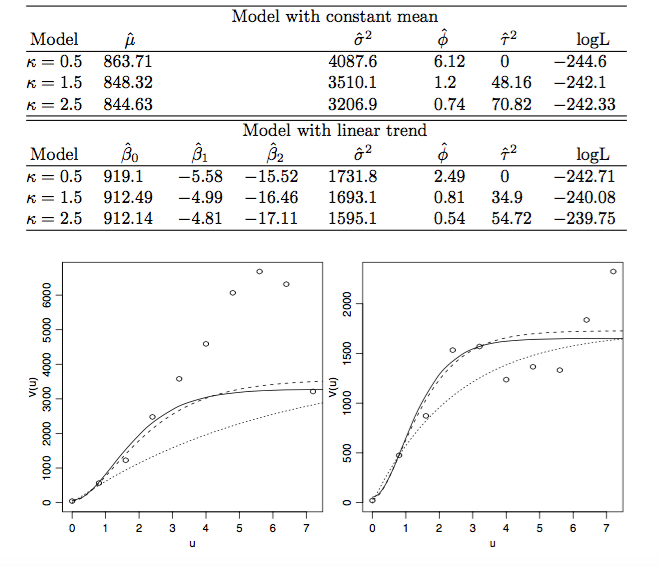
\includegraphics[scale = 0.45]{Images/Pic1}
	\end{figure}
	
\end{frame}

\section{Extension - Preferential Sampling}

\begin{frame}{Preferential Sampling}
\begin{block}{The Problem}
\begin{itemize}
\item So far we have assumed the sampling locations $X$ are fixed, or assumed known.
\item What if the sampling locations depend on the underlying field $S$?
\end{itemize}
\end{block}

\begin{example}
\begin{itemize}
\item Pollution data from measuring stations
\item Ocean temperature data from marine mammals
\item Lead concentration in Galicia (to be shown)
\end{itemize}
\end{example}
\end{frame}

\begin{frame}{Preferential Sampling}

\begin{figure}
\centering
\caption{Example of a single realisation of $S$ and corresponding 100 sampling locations selected using a spatial Poisson Process with intensity $\lambda(x)=\exp(\beta S(x))$.\label{fig:PrefSimPlot}}
\subfigure[Example of 100 preferentially sampled locations ($\beta=2$)]{\label{fig:a}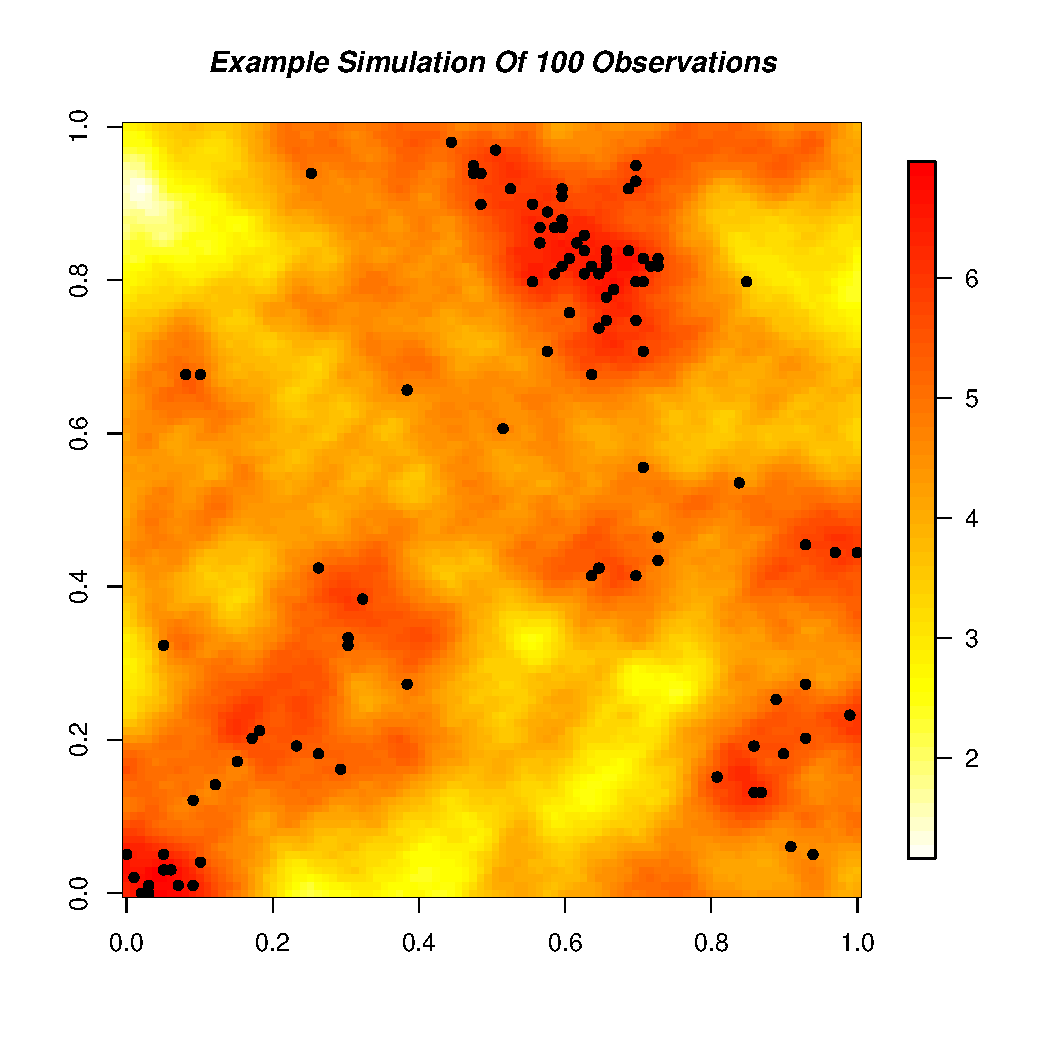
\includegraphics[width=50mm]{Images/DiggleFakeSimPlot.pdf}}
\subfigure[Example of 100 non-preferentially sampled locations ($\beta=0$)]{\label{fig:b}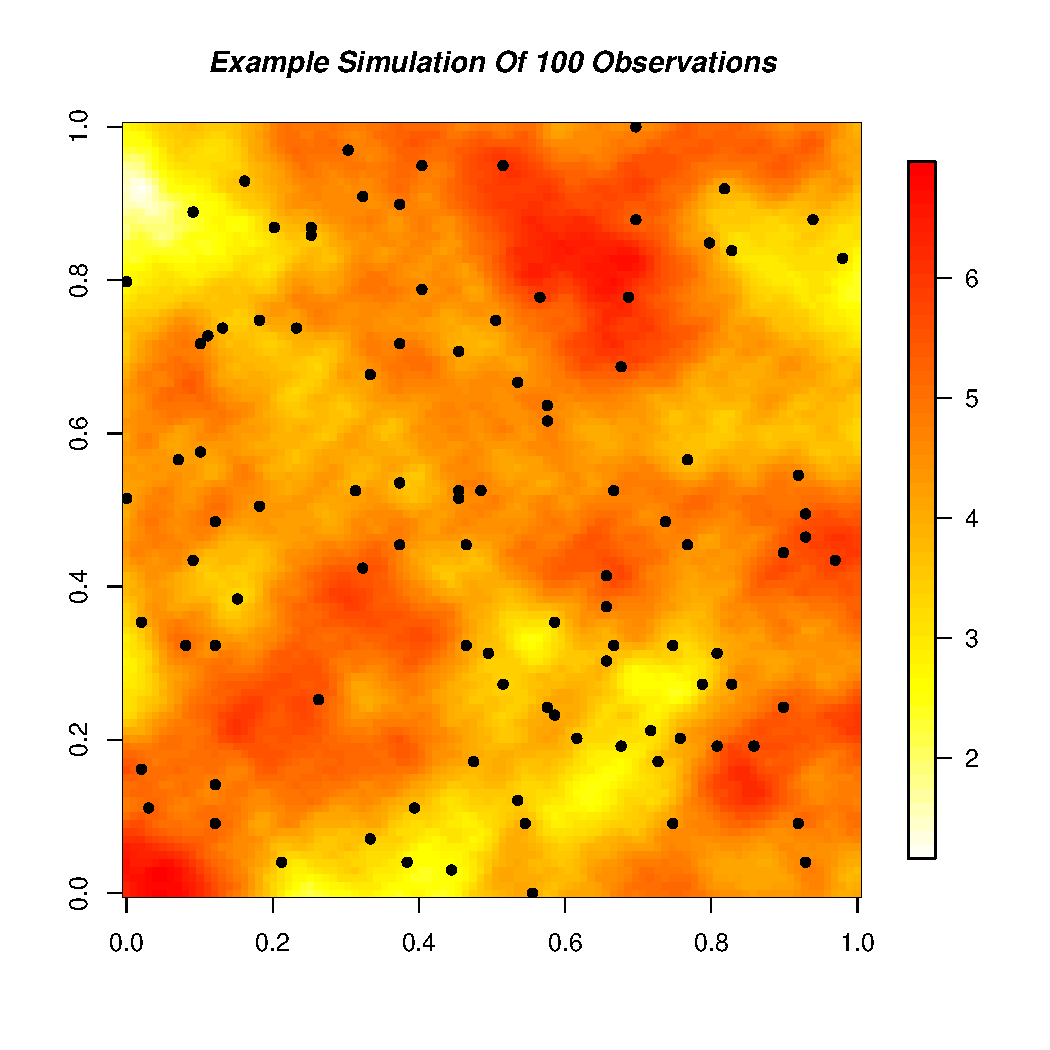
\includegraphics[width=50mm]{Images/DiggleFakeSimPlotNP.pdf}}
\end{figure}
\end{frame}

\begin{frame}{Preferential Sampling}
\begin{block}{Solution}
\begin{itemize}
\item We must account for the dependence between $X$ and $S$.
\begin{equation}
L(\boldsymbol{\theta})=\int \left[X,Y,S\right]\mathrm{d}S.
\end{equation}
\item Diggle et al. 2010 - Monte Carlo 
\item Integrated Nested Laplace Approximation (INLA) - Joe
\item Template Model Builder - Danny
\end{itemize}
\end{block}
\end{frame}

\begin{frame}{Preferential Sampling}
\begin{block}{Results}
\small
\begin{table}[ht]
\centering
    \begin{tabular}{| c | c | c | c | c |}
    \hline
    Model & Parameter  & Standard MLE & {\it TMB} \\ \hline
    Preferential & Bias & (0.77, 1.36)  & (0.41, 0.94) \\
    Preferential & Root-mean-square error & (0.86, 1.40) & (0.60, 1.05)  \\ \hline
\end{tabular}
    \caption {Comparison of approximate $95\%$ confidence intervals for the root-mean-square errors and bias between standard MLE and {\it TMB} over 50 independent simulations for preferential ($\beta=2$) at location $x_0=(0.49, 0.49)$.}
 \label{table:simtable}
\end{table}
\normalsize
\end{block}

\end{frame}
% Placing a * after \section means it will not show in the
% outline or table of contents.
\section*{Summary}

\begin{frame}{Summary}
  \begin{itemize}
  \item
    The \alert{first main message} of your talk in one or two lines.
  \item
    The \alert{second main message} of your talk in one or two lines.
  \item
    Perhaps a \alert{third message}, but not more than that.
  \end{itemize}
  
  \begin{itemize}
  \item
    Outlook
    \begin{itemize}
    \item
      Something you haven't solved.
    \item
      Something else you haven't solved.
    \end{itemize}
  \end{itemize}
\end{frame}



% All of the following is optional and typically not needed. 
\appendix
\section<presentation>*{\appendixname}
\subsection<presentation>*{For Further Reading}

\begin{frame}[allowframebreaks]
  \frametitle<presentation>{For Further Reading}
    
  \begin{thebibliography}{10}
    
  \beamertemplatebookbibitems
  % Start with overview books.

  \bibitem{Author1990}
    A.~Author.
    \newblock {\em Handbook of Everything}.
    \newblock Some Press, 1990.
 
    
  \beamertemplatearticlebibitems
  % Followed by interesting articles. Keep the list short. 

  \bibitem{Someone2000}
    S.~Someone.
    \newblock On this and that.
    \newblock {\em Journal of This and That}, 2(1):50--100,
    2000.
  \end{thebibliography}
\end{frame}

\end{document}




